\section{Fases}
\subsection{Fase 1}
O cenário geral representa uma floresta de coníferas. Esta será dividida em quatro 
regiões: A, B, C e D, tal como ilustrado na Figura 2. A região A localiza-se na parte 
mais alta da floresta, onde encontra-se a tribo do personagem principal e é a posição 
que este inicia no jogo. Para deslocar-se entre as regiões A e B, o personagem deverá 
descer a montanha saltando entre as pedras. O personagem deverá morrer em caso de 
quedas altas. Como dificuldade de percurso, haverá pedras soltas que exigirão rapidez 
do jogador. Esta região de transição também estará infestada de cobras. A região B 
será plana e composta por muitas árvores. Esta área será dominada por ursos e em 
algumas árvores haverá cachos de abelhas. Na região C há um rio repleto de jacarés. 
O personagem poderá atravessá-lo andando (não correndo), já que as águas são baixas, 
ou pulando sobre as pedras no rio. Por fim, na região D, é onde encontra-se o último 
inimigo do personagem, o tigre.

\begin{figure}[!ht]
 \centering
 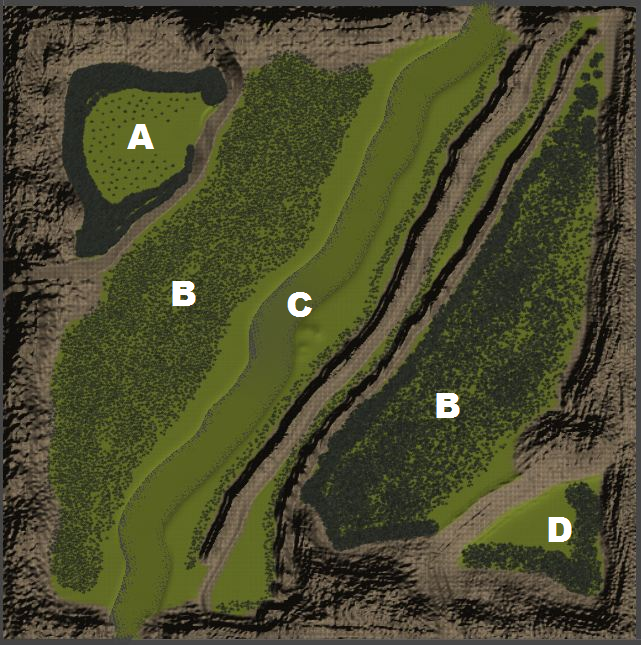
\includegraphics[scale=0.6]{cenario01.png}
 \caption{Esboço do cenário geral da primeira fase.}
 \label{img:reason}
\end{figure}